%%%%%%%%%%%%%%%%%%%%%%%%%%%%%%%%%%%%%%%%%%%%%%%%%%%%%%%%
%%%%%%%%%%%%%%%%%%%%%%%%%%%%%%%%%%%%%%%%%%%%%%%%%%%%%%%%
\section{Materials and Methods}
\label{sec:materials_and_methods}
%%%%%%%%%%%%%%%%%%%%%%%%%%%%%%%%%%%%%%%%%%%%%%%%%%%%%%%%
%%%%%%%%%%%%%%%%%%%%%%%%%%%%%%%%%%%%%%%%%%%%%%%%%%%%%%%%
%
OWP FIM is a fully operational pipeline of software tools to help acquire datasets, cache hydrofabrics, produce FIMs, and evaluate results.
Figure \ref{fig:methods_overview} gives a high level overview of the methodology used in OWP FIM and in this study.
Input data from multiple sources are preprocessed (not illustrated) and then subset to processing areas based on the model used, FR, MS, or GMS.
The standard processing unit of OWP FIM is a HUC8 and the entire NWM FR stream network is used for enforcment.
Later, we explain how only the NWM MS stream network is used for the MS version of HAND, while for GMS, the FR stream network is discretized into LPs before computing HAND.
A series of hydro-conditioning steps enforces the location of stream lines, monotonically decreasing elevations, excavated bathymetry, stream thalweg breaching, and levee enforcement.
After a DEM suitable for HAND's assumptions is conditioned, the FIM hydrofabric is generated including stream network, catchments, HAND, SRCs, and cross-walk table.
The FIM hydrofabric is defined as the datasets required to make an inundation map from discharges including the relative elevation model (REM) or HAND grid, the catchments in vector and raster form, and the hydro-table (contains SRC and cross-walk information).
In operational circumstances, the NWM streamflows are used in conjunction with the FIM hydrofabric to derive forecast FIMs.
However for evaluation purposes, we use the streamflows from the cross-sections of our benchmark model.
As later discussed in Section \ref{ssec:inundation_mapping}, independent FIMs from multiple fluvial sources are mosaiced together.
For the case of MS, two sources are mosaiced together (FR and MS) while for GMS the inundation from every LP is composited together.
The evaluation FIM extents are compared to the extents of the benchmark model and metrics are computed.
%
\begin{figure}[H]
\centering
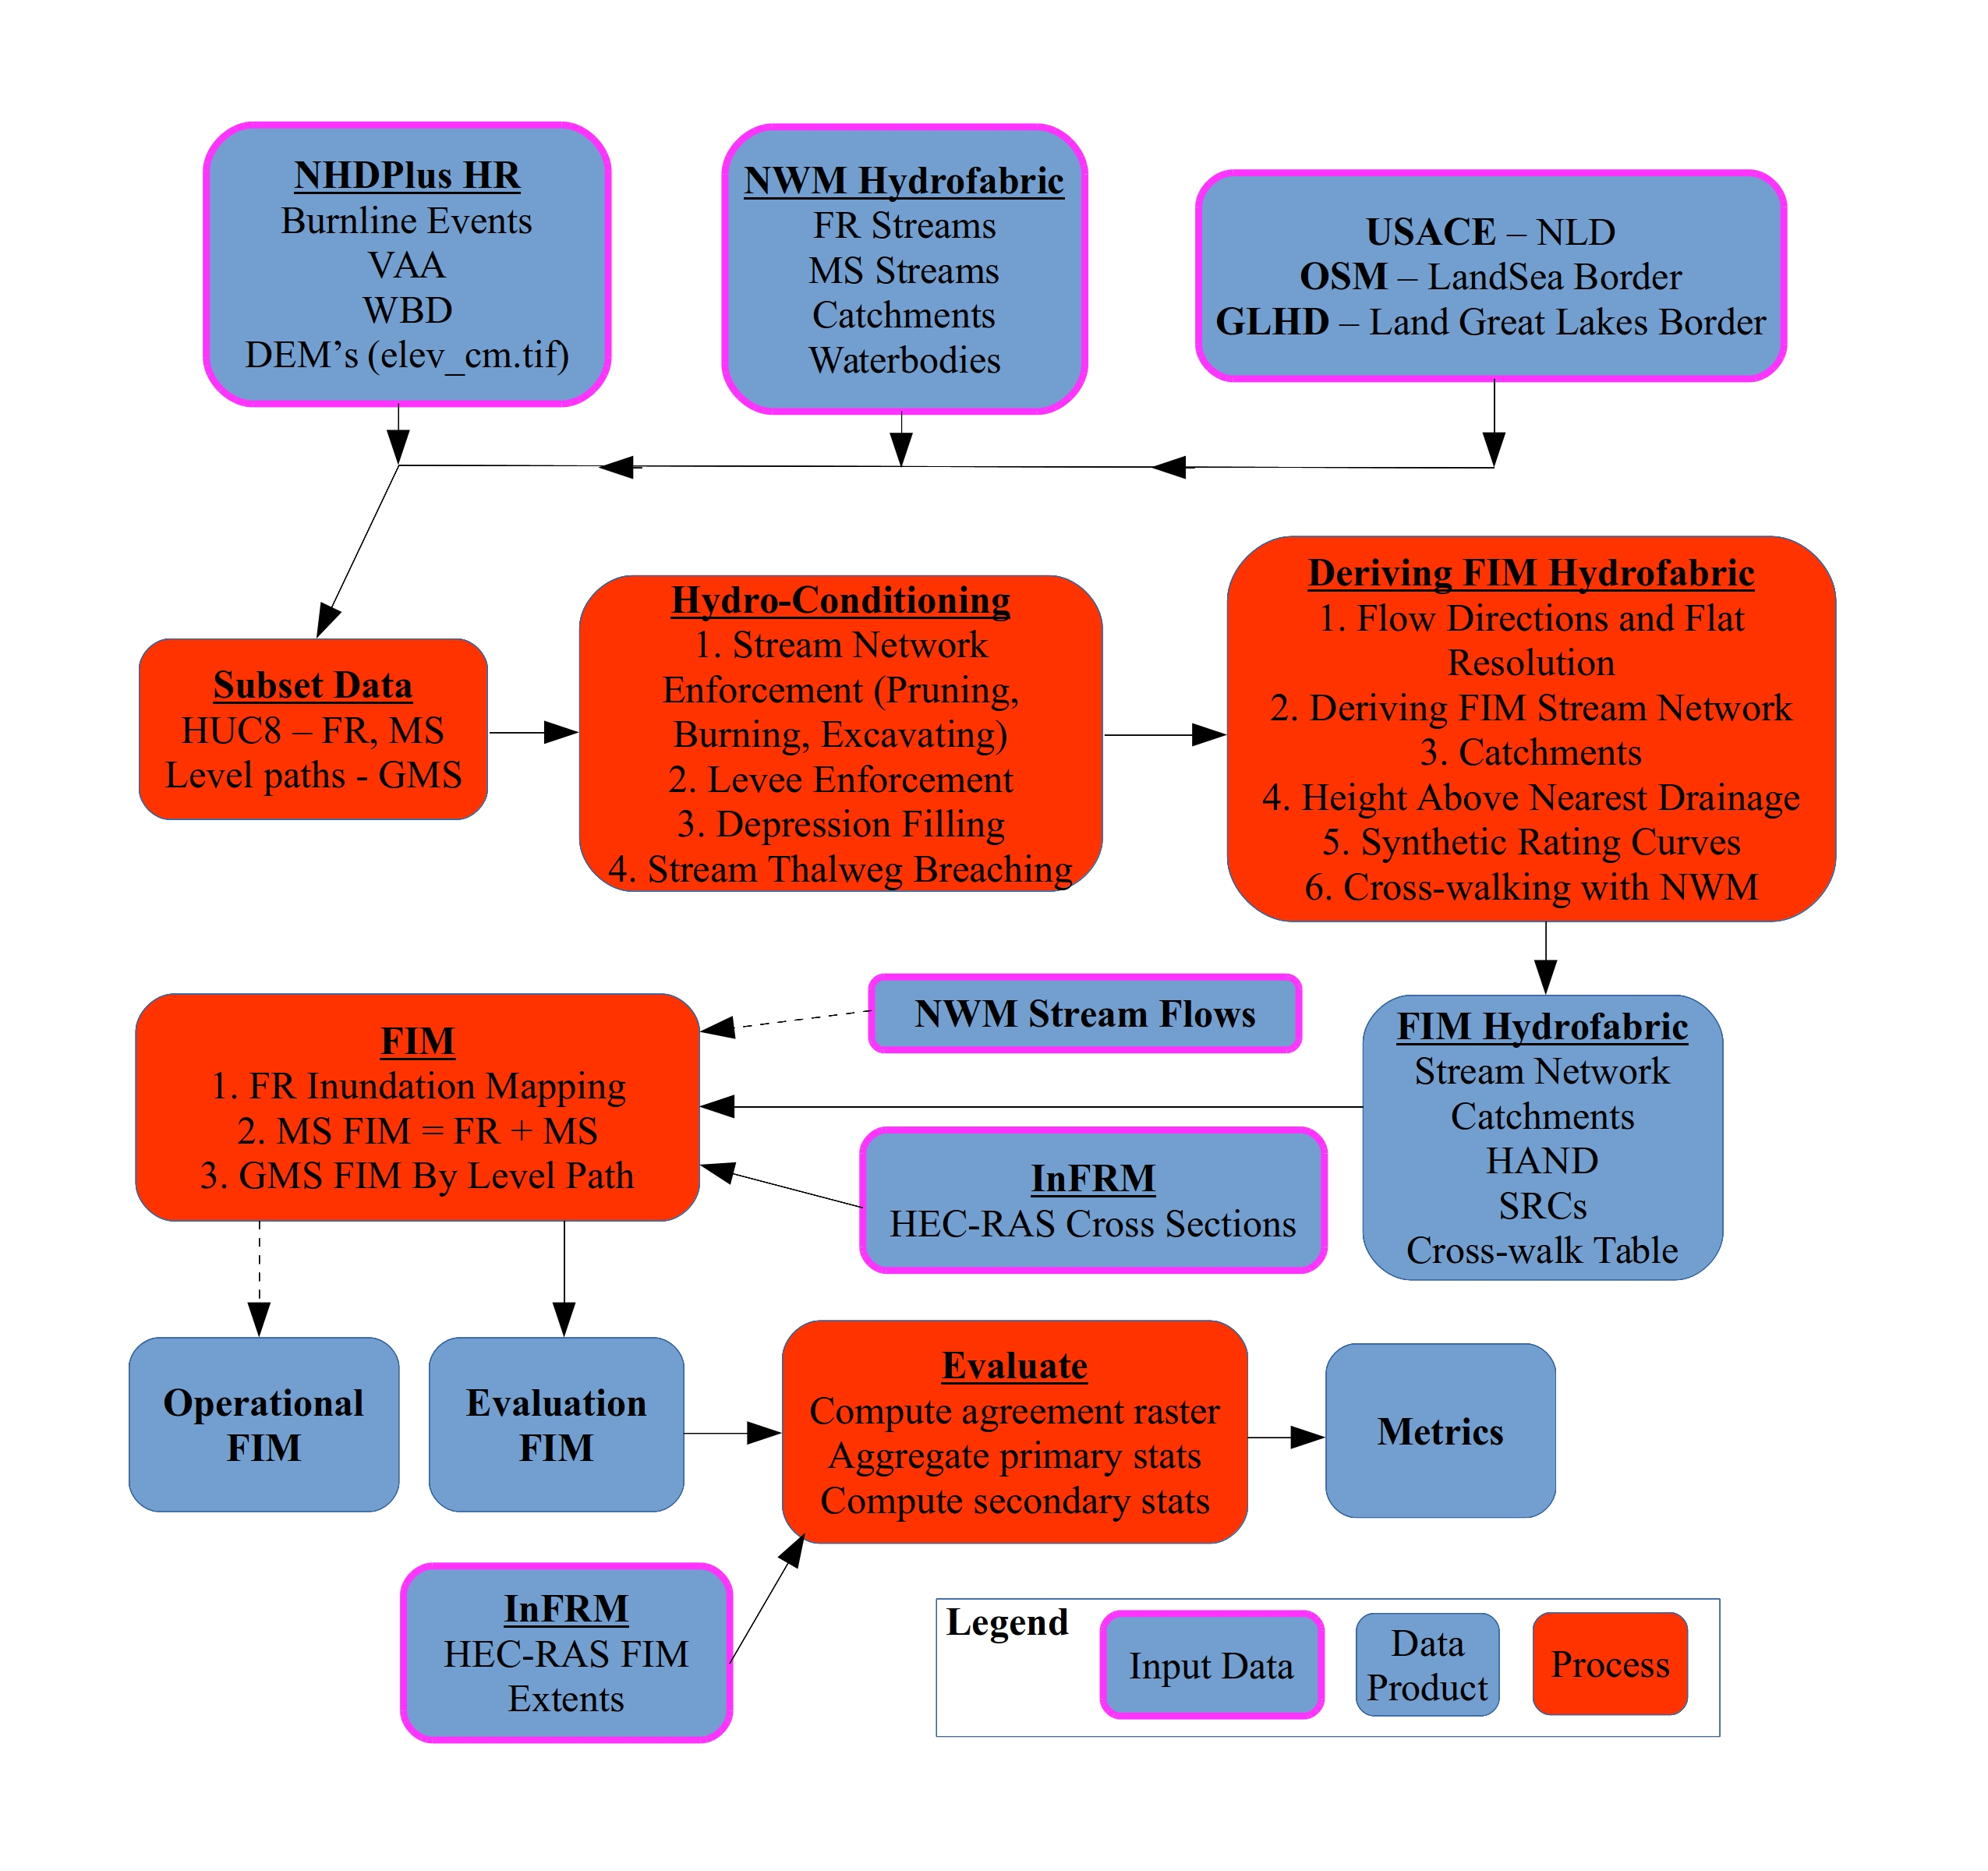
\includegraphics[scale=6.0]{figures/methods_overview.jpg}
\caption{
Methodology overview detailing high level steps followed in the study.
The flow chart begins with the input data organized by source.
Subsetting the data into processing units depends on which model is being considered.
FR utilizes the entire NWM stream network processed at HUC8 processing areas.
MS only computes HAND using the NWM stream at or downstream of legacy forecasting points.
The resulting inundation from the MS HAND is eventually layered with the FIM from FR HAND to account for high levels of inundation contributed by the mainstem.
Generalized Mainstem (GMS) discretized NWM streams into level paths (LP) then computes HAND and the FIMs independently only to mosaic them later. 
This better accounts for multiple possible sources of fluvial inundation.
The dotted lines denote the use of NWM streamflow forecasts to produce operational FIM but not used in this study.
All acronyms used in the figure are defined in the paper.
}
\label{fig:methods_overview}
\end{figure}
%
%
%%%%%%%%%%%%%%%%%%%%%%%%%%%%%%%%%%%%%%%%%%%%%%%%%%%%%%%%
\subsection{Software Dependencies and Architecture}
\label{ssec:software}
%%%%%%%%%%%%%%%%%%%%%%%%%%%%%%%%%%%%%%%%%%%%%%%%%%%%%%%%
%
OWP FIM exclusively utilizes free and open source software dependencies including Python 3, GDAL, TauDEM, Geographic Resource Analysis Support System (GRASS), GNU Parallel, and MPICH \cite{python382,gdal2020,tarboton2005terrain,grass2020,tange2015gnu,amer2021mpich}.
Within the Python 3 ecosystem, many common packages are employed including but not limited to RichDEM, GeoPandas, Rasterio, Rasterstats, and Numba \cite{barnes2018richdem,jordahl2014geopandas,lam2015numba}. 
To simplify setup and enhance portability across host operating systems, OWP FIM packages all dependencies up in a Docker image \cite{merkel2014docker}. 
A user only needs to install Docker on their host machine and build the image from the provided recipe. 
Source code is made available for this project on GitHub where a user could consult the Readme.md page for more information on how to acquire the datasets and reproduce the pipeline \cite{inundationMapping2022}.
%
%%%%%%%%%%%%%%%%%%%%%%%%%%%%%%%%%%%%%%%%%%%%%%%%%%%%%%%%
\subsection{Datasets}
\label{ssec:datasets}
%%%%%%%%%%%%%%%%%%%%%%%%%%%%%%%%%%%%%%%%%%%%%%%%%%%%%%%%
%
Data sources used within OWP FIM are publicly available from a variety of government sources including the USGS, NWC, Federal Emergency Management Agency (FEMA), and US Army Core of Engineers (USACE) to enhance reproducibility and collaboration among government, academia, and industry.
Instructions for accessing data processed for OWP FIM are provided on the project's GitHub page via an Amazon Web Services (AWS) S3 bucket furnished by the Earth Science Information Partners (ESIP) \cite{esipData2022}.
The National Hydrography Dataset Plus High Resolution (NHDPlusHR) Beta Version is the latest hydrography dataset used for land surface hydrologic modeling in the US \cite{moore2019user}.
We utilized a series of data products from the NHDPlusHR including the BurnLineEvents \cite{nhdplus2022vectors}, Value Added Attributes (VAA) \cite{nhdplus2022vectors}, Water Boundaries (WBD) or HUC Layers \cite{nhdplus2022wbd}, and the DEM elevation rasters \cite{nhdplus2022dems}.
These BurnLines used in conjunction with the hydrofabric of the NWM V2.1 to help define flowlines for OWP FIM while the NWM hydrofabric is also used to define reservoirs for exclusion and catchments to cross-walk against for forecasting purposes \cite{nwm2022hydrofabric}.
For enforcing levee data, the USACE NLD is used to burn feature elevations into DEMs \cite{engineers2016national}.
Since NHDPlusHR datasets extend beyond land borders into sea and Great Lake regions, we used the land-sea border from OpenStreetMap (OSM) \cite{osm2021landsea} and the land-lake border from Great Lakes Hydrography Dataset (GLHD) \cite{GreatLakesHydrographyDataset} to exclude those areas from production of FIMs.
Additionally, the Base Level Engineering (BLE) datasets within FEMA Region 6 spanning parts of nine states including Colorado, New Mexico, Texas, Oklahoma, Kansas, Arkansas, Louisiana, Missouri and Mississippi at two recurrence intervals, 1\% (100 year or yr) and 0.2\% (500 year or yr), are used for validation in this study and furnished by the Interagency Flood Risk Management (InFRM) consortium \cite{fema2021base,fema2021estimated}. 
These BLE datasets are provided at the watershed scale (HUC8) utilizing best available DEMs and simulations from the Hydrologic Engineering Center's River Analysis System (HEC-RAS) model \cite{us2022hydrologic}.
The full input datasets presented by source are listed in Table \ref{tab:data}.
%
\begin{sidewaystable}
\caption{Data sources, names, descriptions, and citations.}
\label{tab:data}
\centering
\begin{tabular}{|p{1.75cm}|p{4cm}|p{11cm}|p{5cm}|}
%\begin{tabular}{l c c}
\hline
Source & Name & Description & Citations\\
\hline
USGS & NHDPlusHR BurnLineEvents & Stream lines used by NHDPlusHR for hydro-enforcement. & \cite{nhdplus2022vectors} \\
\hline
USGS & NHDPlusHR Value-Added Attributes & Database of additional attributes associated with the BurnLineEvents that enhance navigation, analysis, and display. & \cite{nhdplus2022vectors} \\
\hline
USGS & NHDPlusHR DEM & DEM used for NHDPlusHR at 1/3 arc-second (10 m) spatial resolution and vertical units in centimeters. & \cite{nhdplus2022dems} \\
\hline
USGS & NHDPlusHR WBD & Water Boundaries (WBD) or HUCs used for spatial processing units. & \cite{nhdplus2022wbd} \\
\hline
NOAA-OWP & NWM Streams & Stream network center lines used by NWM for routing and forecasting adapted from NHDPlus V2 NHDFlowline\_Network feature class. & \cite{nwm2022hydrofabric} \\
\hline
NOAA-OWP & NWM Catchments & Surface drainage area corresponding to each reach in the NWM adapted from NHDPlus V2 Catchment feature class. & \cite{nwm2022hydrofabric} \\
\hline
NOAA-OWP & NWM Waterbodies & Waterbodies considered by the NWM as reservoirs or lakes adapted from NHDPlus V2 NHDWaterbody feature class. & \cite{nwm2022hydrofabric} \\
\hline
USACE & NLD & Levee database of locations and elevations. & \cite{engineers2016national} \\
\hline
OSM & Land-Sea Border & Border of land and sea. & \cite{osm2021landsea} \\
\hline
GLHD & Land-Great Lakes Border & Border of land and Great Lakes. & \cite{GreatLakesHydrographyDataset} \\
\hline
InFRM & Cross-Sections & HEC-RAS 1D cross-sections used for modeling in BLE datasets. Includes discharges for 1\% and 0.2\% recurrence interval events. & \cite{fema2021estimated} \\
\hline
InFRM & Flood Inundation Extents & Inundation extents produced by InFRM BLE HEC-RAS 1D for 1\% and 0.2\% recurrence interval events. & \cite{fema2021estimated} \\
\hline
\end{tabular}
%\end{table}
\end{sidewaystable}
%
Areas with all the required data (from the NWM and the USGS) are labeled as the FIM domain which includes 2,188 HUC8s for the FR and GMS networks and 1,604 HUC8s for the MS method. 
These methods will be explained in more detail later.
An enhancement of OWP FIM over previous HAND based FIM versions is the support for Hawaii and Puerto Rico which are expansion domains in the NWM V2.0 and V2.1, respectively.
%
%%%%%%%%%%%%%%%%%%%%%%%%%%%%%%%%%%%%%%%%%%%%%%%%%%%%%%%%
\subsection{Hydro-conditioning}
\label{ssec:hydro_conditioning}
%%%%%%%%%%%%%%%%%%%%%%%%%%%%%%%%%%%%%%%%%%%%%%%%%%%%%%%%
%
The DEM is subject to a series of hydro-conditioning procedures to enhance its suitability for riverine flood inundation mapping with HAND. 
These techniques are specific for making OWP FIM and differ from the conditioning methods used by the NHDPlusHR Beta \cite{moore2019user}.
HAND inherently requires all areas eligible for inundation to drain to the designated drainage network.
So to satisfy this requirment, DEMs must undergo significant manipulation.
In other words, all areas within a given processing unit for HAND must have monotonically decreasing elevations to enable eligiblity for flooding.
Hydro-conditioning is implemented to obtain many objectives including enforcing the location of hydrologically relevant features such as flowlines, lakes, or drainage divides whether natural or anthropogenic. 
It can also be used to simulate more accurate bathymetry which is not accounted for in the 10 m DEM \cite{gesch2002national}.

Specifically within the context of OWP FIM, the hydro-conditioning operations that take place in sequential order are presented. 
Prior to any hydro-conditioning, all input datasets must be subset from their original spatial domain scales into the processing units of size HUC8. 
The subsetting is done by spatial query for the cases of the levees, DEM, and NWM hydrofabric while the NHDPlusHR BurnLineEvents are subset via attribute query for the given reach code's membership in the processing unit.
Hydro-conditioning raster operations take place on buffered boundary definitions to avoid edge contamination and effects \cite{lindsay2013measuring}. 
%
%%%%%%%%%%%%%%%%%%%%%%%%%%%%%%%%%%%%%%%%%%%%%%%%%%%%%%%%
\subsubsection{Stream Network Enforcement} 
\label{ssec:stream_network_enforcement}
%
Both the location and geometry of the stream network are enforced to agree with the NWM stream network and to enforce synthetic bathymetry and generate more hydrologically correct catchments.
The NHDPlusHR Beta BurnLineEvent layer is used to enforce stream locations in the NHDPlusHR workflow and best agrees with thalweg locations in the DEM used so it is also used here for hydro-enforcement \cite{moore2019user}. 
This network goes through a stream density reduction procedure to better match the stream density of the NWM stream network.
This reduced density NHDPlusHR network is now used for hydro-enforcement along with the AGREE DEM Surface Reconditioning System to excavate channels into the DEM \cite{hellweger1997agree}.
Downsides to the technique include the possibility of exhibiting parallel streams where the burned stream and real stream are both represented \cite{hellweger1997agree,saunders1999preparation} and some distortion of the catchment boundaries can also be observed \cite{saunders1999preparation,saunders1996gis}.
Some of these drawbacks are addressed by additional conditioning techniques applied later on.
For more details on how we reduce the density of the NHDPlusHR stream network along with technical implementation information on the AGREE DEM procedure, please see \ref{sec:app_stream_network_enforcement}.
%
%%%%%%%%%%%%%%%%%%%%%%%%%%%%%%%%%%%%%%%%%%%%%%%%%%%%%%%%
\subsubsection{Levee Enforcement}
%
Coarse DEM's at 10 m, 30 m, and higher resolutions can lack sufficient representation of fine grain features such as embankments, flood walls, and closure structures \cite{arundel2018assimilation,dobbs2010evaluation,wang2005comparison,sanders2007evaluation}.
In order to better represent the influences of these features upon hydraulics and inundation extents, the National Levee Database (NLD) published by USACE was used to enforce elevations within the 1/3 arc-second DEM.
The elevations found in the NLD are burned onto the DEM if those elevations were found to exceed those already in place.
%
%%%%%%%%%%%%%%%%%%%%%%%%%%%%%%%%%%%%%%%%%%%%%%%%%%%%%%%%
\subsubsection{Depression Filling}
\label{sssec:depression_filling}
%
Local depressions are naturally occurring features of a DEM but must be addressed if a connected drainage network with continuous catchments are to be derived for flood modeling purposes with HAND.
The partially conditioned DEM was removed of depressions by filling areas with pits while preserving the stream and levee information previously enforced.
Priority-Flood developed by \citeA{barnes2014priority} is an algorithm for filling said depressions and shown to have improved performance over early works in the field by \citeA{jenson1988extracting} implemented in \citeA{tarboton2005terrain} as well as \citeA{planchon2002fast}.
The depression filling algorithm used in our pipeline is a Priority-Flood variant developed by \cite{zhou2016efficient} with enhanced single-thread performance and a time complexity of O(n log n) for floating point grids.
This performance was enabled by limiting the processing queue with a region-growing method to exclude many of the slope cells \cite{zhou2016efficient}.
The depression filling technique employed here does leave the existence of flat regions where pits previously existed thus later requiring the need for resolving these flats.
The enhanced variant of Priority-Flood is implemented and made available by \citeA{barnes2018richdem} and \citeA{zhou2015filldem}.
%
%%%%%%%%%%%%%%%%%%%%%%%%%%%%%%%%%%%%%%%%%%%%%%%%%%%%%%%%
\subsubsection{Stream Thalweg Elevation Conditioning}
\label{sssec:stream_thalweg_elevation_conditioning}
%
Thalweg elevations are critical components of relative elevation based inundation mapping thus much is performed to ensure the best available, monotonically decreasing, elevations are derived prior to the normalizing of elevations.
Work on the AGREE DEM method from several authors have illustrated that the AGREE DEM method does not prevent situations where the burned thalweg and the thalweg endemic to the DEM run parallel to one another \cite{hellweger1997agree,baker2006comparison,saunders1999preparation,saunders1996gis,quenzer1998gis,saunders1995grid}.
These works observe that the artificial elevations enforced by the hydrographically based stream network and AGREE DEM disagree with those naturally occurring in the native DEM.
In order to mitigate this documented issue, the normalized excavation algorithm \cite{saunders1999preparation} is used to seek a zonal (nearest neighbor) elevation minimum on the original, unconditioned DEM for each thalweg pixel. 
Each zone is defined as the thalweg's pixel nearest neighborhood within a maximum distance of 50 m.
The zonal minimum is computed for each thalweg pixel zone and the minimum is used to replace the existing thalweg elevation value.
This step essentially enforces an estimate of the native DEM thalweg elevations onto the sharp drop enforced thalweg elevations from the AGREE procedure.

The next step involves conditioning these local minimums along the thalweg to enforce monotonically decreasing thalweg elevations for FIM.
\citeA{garousi2019terrain} proposed an algorithm that breaches stream thalweg pixel elevations in a depth first manner. 
This procedure was found to increase the Critical Success Index (CSI) of resulting FIMs from HAND and is employed in OWP FIM to enforce monotonically decreasing elevations with thalweg pixel networks.
%
%%%%%%%%%%%%%%%%%%%%%%%%%%%%%%%%%%%%%%%%%%%%%%%%%%%%%%%%
\subsection{Deriving FIM Hydrofabric}
\label{ssec:deriving_fim_hydrofabric}
%%%%%%%%%%%%%%%%%%%%%%%%%%%%%%%%%%%%%%%%%%%%%%%%%%%%%%%%
%
The FIM Hydrofabric is defined here as the collection of geospatial datasets that are used for converting NWM discharges into inundation extents.
These datasets include the HAND or relative elevation model (REM) raster, reach-level catchments raster/polygons, DEM-derived streamlines, SRCs, and cross-walk table.
Within the context of this section, we refer to HAND as a grid of relative elevations to detrend elevations away from mean level towards elevations referenced to the nearest drainage line (See Section \ref{sssec:hand}).
SRCs are considered stage-discharge relationships that are derived synthetically using the Manning's equation (See Section \ref{sssec:synthetic_rating_curve}).
Lastly, a cross-walk table attempts to conflate NWM reach identifiers to those derived of the FIM stream network (See Section \ref{sssec:cross_walking_networks}).
The following sub-sections describe how the subset and hydro-enforced geospatial datasets are converted into the FIM hydrofabric.
%
%%%%%%%%%%%%%%%%%%%%%%%%%%%%%%%%%%%%%%%%%%%%%%%%%%%%%%%%
\subsubsection{Flow Directions and Flats Resolution}
\label{ssec:flow_direction_and_flat_resolution}
%
To facilitate the generation of a connected stream network and its associated catchments from the conditioned DEM, the depression-filled DEM is used to derive connectivity in the form of D-8 flow directions \cite{o1984extraction}.
Flat resolution from flats endemic to the DEM or from depression filled regions is a costly, non-trivial procedure which was originally addressed by \citeA{garbrecht1997assignment} where flats are resolved by incrementing elevations iteratively.
OWP FIM utilized a CyberGIS implementation of the D-8 flow direction algorithm with the accelerated resolution of flats which we found to be very efficient and effective \cite{survila2016scalable,cybergis2016}.
For more information on the derivations of flow directions and resolving flats, please see \ref{sec:app_flow_direction_and_flat_resolution}.
%
%%%%%%%%%%%%%%%%%%%%%%%%%%%%%%%%%%%%%%%%%%%%%%%%%%%%%%%%
\subsubsection{Deriving FIM Stream Network}
\label{sssec:deriving_fim_stream_network}
%
The derivations of relative elevations and catchments from the newly conditioned DEM involves re-deriving a new, DEM based, FIM stream network. 
The FIM stream network is of similar drainage density as the NWM V2.1 network and fully converges at all junctions leaving no divergences in the network.
This is accomplished by using the seed points generated from the stream network enforcement process (Section \ref{ssec:stream_network_enforcement} and \ref{sec:app_stream_network_enforcement}).
These seeds points are headwater locations of the NHDPlusHR Beta BurnlineEvents layer that spatially correspond to the headwater definitions in the stream network of the NWM V2.1.
Feeding the seed points and previously computed flow directions into flow accumulation methods \cite{wallis2009parallel,tarboton1997new,tarboton2005terrain} yields a stream link accumulation raster that can be converted to a vector file for further processing.

Each stream link in this derived FIM stream network is split into equidistant reaches of 1.5 km in length which is a user exposed parameter.
Stream links are defined here as segments of rivers discretized by junctions with other NWM river segments.
Stream links are then further segmented at NWM lakes and HUC8 boundaries.
Discretizing at NWM lakes isolates reaches and catchments associated with lakes and reservoirs to avoid mapping them using the Manning's equation and could potentially enable volume based mapping in the future as a feature enhancement.
Based on previous research, splitting each remaining stream link into equidistant reaches not to exceed a parameterized value of 1.5 km helps improve SRC and mapping skill \cite{garousi2019terrain,godbout2019error,zheng2018geoflood}.
This parameter was held constant across all versions of HAND that we used which are introduced in Section \ref{ssec:stream_order_reduction}.
Small reaches can lead to unrealistic variances in channel geometries while oversized reaches can lead to grouping too much slope variance into one discretization of the stream network.
Short stream segments that are introduced as a result of forced network breaks due to reservoir, levee, or HUC boundaries inherit the SRC properties of the upstream or downstream segment, depending on the topology.
Section \ref{sssec:synthetic_rating_curve} details the derivation of the SRC and the dependence on channel length. 
Additionally every reach (and later catchment) is assigned a globally unique identifier based on the HUC8 membership.
This stream network is important since it drives the HAND calculation and derivation of catchments.
%
%%%%%%%%%%%%%%%%%%%%%%%%%%%%%%%%%%%%%%%%%%%%%%%%%%%%%%%%
\subsubsection{Catchments}
\label{sssec:catchments}
%
Catchments were derived using the D8 connectivity established by \citeA{o1984extraction}.
Outlet points are set at the pixel center points of the delineated stream lines explained in Section \ref{sssec:deriving_fim_stream_network}.
The outlets act as root nodes in a tree structure and the connectivity is traversed to derive the contributing, nearest drainage region for each outlet point.
Two sets of catchments are derived, one set of catchments denotes the unique drainage region for each thalweg pixel which is used for relative elevation calculation.
The other catchments are derived for the drainage region for each stream reach as defined in Section \ref{sssec:deriving_fim_stream_network}. 
%
%%%%%%%%%%%%%%%%%%%%%%%%%%%%%%%%%%%%%%%%%%%%%%%%%%%%%%%%
\subsubsection{Height Above Nearest Drainage}
\label{sssec:hand}
%
Once the pixel level catchments are derived, the final relative elevations can be computed.
To compute these relative elevations, we utilize the same technique found in previous HAND implementations \cite{zheng2018geoflood,zheng2018river,nobre2011height,nobre2016hand,maidment2017conceptual,garousi2019terrain}.
For each pixel level catchment described in Section \ref{sssec:catchments}, we subtract the elevations of the non-thalweg pixels from the thalweg pixel of that catchment.
Contrary to some of the some other previous HAND implementations, the DEM used for this operation is the DEM resulting from the thalweg conditioning procedures described in Section \ref{sssec:stream_thalweg_elevation_conditioning} \cite{djokic2019arc}.
This DEM utilizes the native elevations in regions outside of the excavated channel from the AGREE DEM method \cite{djokic2019arc}.
Any negative values resulting from this subtraction with native elevations are replaced by zero.
Again, HAND assumes and requires processing areas to drain thus have monotonically decreasing elevations with hydrologically correct flow directions all leading to a singular outlet point.
While this is required for the generation of DEM-derived catchments and stream lines, it is not necessarily required for the computation of the relative elevations.
Since the use of hydro-conditioning processes to fit the drainage requirement for HAND can be extensive, we found it more fitting to use the native elevations this final HAND computation thus avoid the use of manipulated values that fit modeling assumptions.
%
%%%%%%%%%%%%%%%%%%%%%%%%%%%%%%%%%%%%%%%%%%%%%%%%%%%%%%%%
\subsubsection{Synthetic Rating Curves}
\label{sssec:synthetic_rating_curve}
%
A method for converting forecast river discharges from the NWM to stages or river depths at the reach scale is necessary for producing FIMs with HAND. 
For 1D hydrodynamic models such as the routing methods in the NWM, the typical procedure is to establish the stage-discharge relationship by sampling data from the DEM to derive a SRC at discrete cross-sections \cite{quintero2021development,di2011hydraulic}. 
For this application, we utilized the reach averaged approach for developing SRCs \cite{zheng2018river}.
The reach averaged approach seeks to sample the geometry parameters in the Manning's equation \cite{gauckler1867etudes,manning1890flow} on a reach scale then dividing those by length. 
Previously not reported in literature to our knowledge in this form, the reach averaged Manning's formula is derived to be 
%
\begin{linenomath*}
\begin{equation}
\label{eq:reach_averaged_mannings_equation}
Q(y) = \frac{1}{n} \frac{V(y)^{5/3}S^{1/2}}{L B(y)^{2/3}} 
\end{equation}
\end{linenomath*}
%
where Q is discharge at stage y, n is the Manning's n roughness coefficient, V is volume at y, S is channel slope, L is the along-flow reach length, and B is wetted bed area at y.
Q, V, and B are taken at specific y values so are more formally written as $Q = Q(y)$, $V = V(y)$, and $B = B(y)$, respectively.
All units are international (SI) given the one in the numerator above n.
The reach averaged method has been compared to rating curves from HEC-RAS and USGS gages yielding comparable results for estimating the river bottom elevation profile, channel width at given stages, and stage-discharge relationships \cite{zheng2018river}.
The reach averaged geometry parameters including number of wet cells, bed area, and volume are sampled from the thalweg conditioned AGREE DEM using TauDEM's catchhydrogeo utility.
Using the split reaches described in Section \ref{sssec:deriving_fim_stream_network}, the channel slope is sampled from the thalweg conditioned DEM at the end points of the reaches while the same reaches are used to calculate the reach length.
While the AGREE DEM is subject to hydro-conditioning processes, it does introduce some notion of bathymetry estimation that the native DEMs lack while being sensitive to additional parameters that could yield further errors in the FIM.
We leave this issue open in this study and elaborate on needs with respect to bathymetry and Manning's n values in the Discussion section (Section \ref{sec:discussion}).
We constrain the equation by selecting 84 stage values (y in Eq. \ref{eq:reach_averaged_mannings_equation}) from 0 to 25 meters in depth at a third of a meter increments to calculate the discharge values for each stage value. 
Due to the varying nature of stage (y in Equation \ref{eq:reach_averaged_mannings_equation}) as explained, the terms V(y) and B(y) also update according to previous work with reach averaged SRCs \cite{zheng2018river}.

Setting of the Manning's n roughness coefficient has precedent in previous continental-scale FIM (CFIM) studies \cite{maidment2017conceptual,liu2016cybergis,liu2020height,djokic2019arc,garousi2019terrain,zheng2018geoflood} with two noted values of 0.05 and 0.06 for NFIE and \citeA{djokic2019arc} respectively. 
These values are applied universally to the entire forecasting domain across space, time, and discharge profiles.
We note significant opportunity to enhance CFIM skill by better localizing Manning's n according to available data including but not limited to land cover, land use, stream order, stream geometry, drainage area, reach length, and discharge percentiles \cite{garousi2019terrain,johnson2019integrated}.
For now and for the purpose of this study, we examine the SRCs with Manning's n set to both 0.06 and 0.12 which we hope will shed some light on the sensitivity of this parameter to HAND based FIMs.
%
%%%%%%%%%%%%%%%%%%%%%%%%%%%%%%%%%%%%%%%%%%%%%%%%%%%%%%%%
\subsubsection{Cross-walking with NWM Stream Network}
\label{sssec:cross_walking_networks}
%
The DEM based stream network derived in Section \ref{sssec:deriving_fim_stream_network} must be associated with NWM reach identifiers so that a discharge can be converted to stage and later inundation extents.
For the FR version of HAND, we overlap the reach catchments derived in Section \ref{sssec:catchments} with the NWM catchments matching the ID of the NWM catchment that most overlaps the derived catchment for HAND.
For two subsequent HAND methods, MS and GMS, discussed in Sections \ref{sssec:nws_mainstems} and \ref{sssec:generalized_mainstems}, respectively, we find the mid-point of the derived stream reach line described in Section \ref{sssec:deriving_fim_stream_network} and find the NWM catchment that contains the mid-point.
Additionally, only relevant catchments from the NWM for the given LP are selected for cross-walking for methods in Sections \ref{sssec:nws_mainstems} and \ref{sssec:generalized_mainstems}.
While these conflation methods are approximate, they can lead to some substantial errors which will be discussed more in Section \ref{sec:discussion}.
%
%%%%%%%%%%%%%%%%%%%%%%%%%%%%%%%%%%%%%%%%%%%%%%%%%%%%%%%%
\subsection{Stream Order Reduction}
\label{ssec:stream_order_reduction}
%
As previously discussed, HAND based FIMs are subject to many assumptions and limitations in order serve as a suitable inundation proxy for large scale, high resolution domains.
As introduced in Section \ref{ssec:owp_fim}, HAND based FIMs fail to account for multiple sources of fluvial inundation which leads to flow constrictions at high flow confluences.
We hypothesized that reducing the scale of HAND computation down to stream networks of unit Horton-Strahler stream order can help account for multiple fluvial sources of inundation.
To clarify the phrase ``reducing Horton-Strahler stream order'' used extensively in this paper, every FIM used in evaluation contains a flood extent sourced from every NWM forecast point in the given evaluation domain.
What we do to reduce stream order is discretize the NWM FR network into different units of size, MS network (\ref{sssec:nws_mainstems}) and GMS LPs (\ref{sssec:generalized_mainstems}), that effectively reduce the HAND computation to independent networks of unit stream order.
These independent HAND datasets are later used to produce FIM independently and mosaiced together (see Section \ref{ssec:inundation_mapping}).
The inundation from the MS HAND is mosaiced with the inundation from FR HAND, while the inundation of each individual LP from GMS is mosaiced together.
The Horton-Strahler stream order is only reduced for HAND computation purposes to reduce the negative effects of the nearest drainage limitation inherent to HAND.
%
%%%%%%%%%%%%%%%%%%%%%%%%%%%%%%%%%%%%%%%%%%%%%%%%%%%%%%%%
\subsubsection{NWS Mainstems}
\label{sssec:nws_mainstems}
%
The initial attempt at drainage order reduction to solve the catchment boundary issue was to use a stream network relevant to the NWS forecasting community. 
The Mainstems (MS) network is a subset of the NWM FR network at and downstream of AHPS forecast points as seen in Figure \ref{fig:forecast_points}.
The MS network comprises about 200 thousand km of stream length which is less than 4\% of the FR total stream length of 5.5 million km.
It also spans 121,724 reaches across 1,608 HUC8s.
In this technique, we derive HAND using the FR stream network as well as the MS network which was originally proposed by \citeA{djokic2019arc}.
Inundation is derived independently from the resulting FR and MS HAND hydrofabrics and are mosaiced together using the technique proposed in Section \ref{ssec:inundation_mapping} to form the MS FIMs. 
Within each HUC, one might typically only find a MS stream network of uniform stream order but this can vary if more than one AHPS forecasting point is found within or upstream of the HUC in question.
So while we may refer to the MS network as that of one with unit stream order, we acknowledge there are many cases where additional or converging forecast points create multiple branches within a given processing unit.
%
%%%%%%%%%%%%%%%%%%%%%%%%%%%%%%%%%%%%%%%%%%%%%%%%%%%%%%%%
\subsubsection{Generalized Mainstems}
\label{sssec:generalized_mainstems}
%
Since MS only covers 4\% of the entire FR stream network, we sought to expand drainage order reduction techniques to all reaches within the NWM modeling domain.
In order to do this, we discretized the NWM network into LPs which when considered individually have unit Horton-Strahler stream orders.
LPs group flowlines by maximizing the length of each flow path and minimizing the number of LP identifiers within a given domain \cite{moore2019user,mckay2012nhdplus}. 
In order to derive LPs for the NWM FR stream network at the HUC8 processing area, we first compute arbolate sums which are defined as the cumulative drainage distance of all upstream drainage lines.
Arbolate sum is also inclusive of the current drainage reach as well.
Arbolate sums are computed by starting at the headwater points and summing up drainage distances as you traverse downstream.

Arbolate sum is critical to discretizing the NWM network into LP identifiers.
Starting at a HUC8's outlet, a unique LP is propagated upstream. 
At every confluence, the direction of maximum arbolate sum is sought to propagate the current LP identifier.
For the remaining parent reaches of the given junction, a new LP identifier is assigned and the process recursively continues with them.
Figure \ref{fig:level_path_methods} illustrates how LPs (symbolized by unique colors) are propagated upstream by the value of arbolate sum.
The figure shows computed arbolate sums and unique LP identifiers on a headwater subset of HUC8 (12020002) for clarity but were computed at the corresponding HUC8.
The mainstem of the figure runs from the red ellipses to the black one which is the outlet.
From the figure, we can see how unique colors are propagated in the direction of the maximum arbolate sum.

Each HUC8 is discretized into LPs independently and the relevant inputs as described in Table \ref{tab:data} are assigned to each LP processing unit given a buffer of seven km.
This buffer was selected to avoid edge contamination \cite{lindsay2013measuring} and to ensure adequate data availability for wide rivers with large catchments in regions with low slope.
Further work could be dedicated to tune this user exposed parameter to better balance its effect on FIM extents and computational expense since larger buffers create additional floating point calculations and storage requirements.
For the time being, we designate this issue to be out of scope.

At the LP scale, the methods in Sections \ref{ssec:hydro_conditioning} and \ref{ssec:deriving_fim_hydrofabric} are executed leaving out any tributaries of the LP in question at the time.
The only exception to this is the use of the NWM stream network directly for use with hydro-enforcement by burning these lines and seeding from its headwater points directly instead of going through the NHDPlusHR network as described in Section \ref{ssec:stream_network_enforcement} and \ref{sec:app_stream_network_enforcement}.
This decision was motivated by the difficulty in deriving LPs in the NWM stream network with high agreement with the LPs derived for the NHDPlusHR stream lines.
We found that the same algorithm to compute arbolate sums and LPs could yield enough disagreements associated with disordered branches or slight differences in arbolate sums that could significantly affect the agreement of the LP identifiers in the NWM and NHDPlusHR networks.
This yielded enough error to justify the use of the NWM directly for hydro-enforcement operations.

Once the NWM FR stream network is discretized into LPs, we independently compute HAND using each LP as the target stream network to be used.
To illustrate the GMS procedure, we reference Figure \ref{fig:gms_methods} to show how deriving HAND and FIMs from GMS works.
In Figure \ref{fig:gms_methods}a, we uniquely color code the LPs derived for the NWM stream network. 
For each one of these lines, we derive HAND and its associated datasets including catchments, crosswalks, and rating curves.
Each LP is buffered to a polygon with a user-exposed, distance parameter of seven km that is used to subset the original DEM for two selected LPs in Figure \ref{fig:gms_methods}b.
We illustrate two HAND grids for two of the LPs in this HUC8 in Figure \ref{fig:gms_methods}c.
Once the FIM hydrofabrics for each LP are generated, we can inundate them individually also shown in Figure \ref{fig:gms_methods}d.
Lastly, these individual FIMs are mosaiced together as explained in Section \ref{ssec:inundation_mapping} and shown in Figure \ref{fig:gms_methods}d.

For a more intimate look at the drainage order reduction procedure GMS, and its effects, we allude to Figure \ref{fig:gms_methods_2} which references the same area (in HUC8 12090301) and set of river junctions as in Figure \ref{fig:catchment_boundaries_issue}.
The catchments and stream lines for HAND computed at the FR scale are illustrated in Figure \ref{fig:gms_methods_2}a where the respective inundation at the 100 yr magnitude is heavily constrained by the limited catchment extents especially at junctions.
In subsequent sub-figures, we show the same datasets for the HAND computation problem for this region but discretized into independent LPs for the main LP (b), the eastern tributary (c), and the western tributary (d).
Notably, inspecting (b), one sees how removing the tributaries creates much larger catchments for the main LP. 
These catchments include drainage areas that would traditionally be considered nearest to the tributaries thus ineligible to receive inundation sourced from the main LP.
The inundation extents in (b) overlap those of (c) and (d) and are mosaiced together by methods explained in Section \ref{ssec:inundation_mapping}.
%
\begin{figure}[H]
\centering
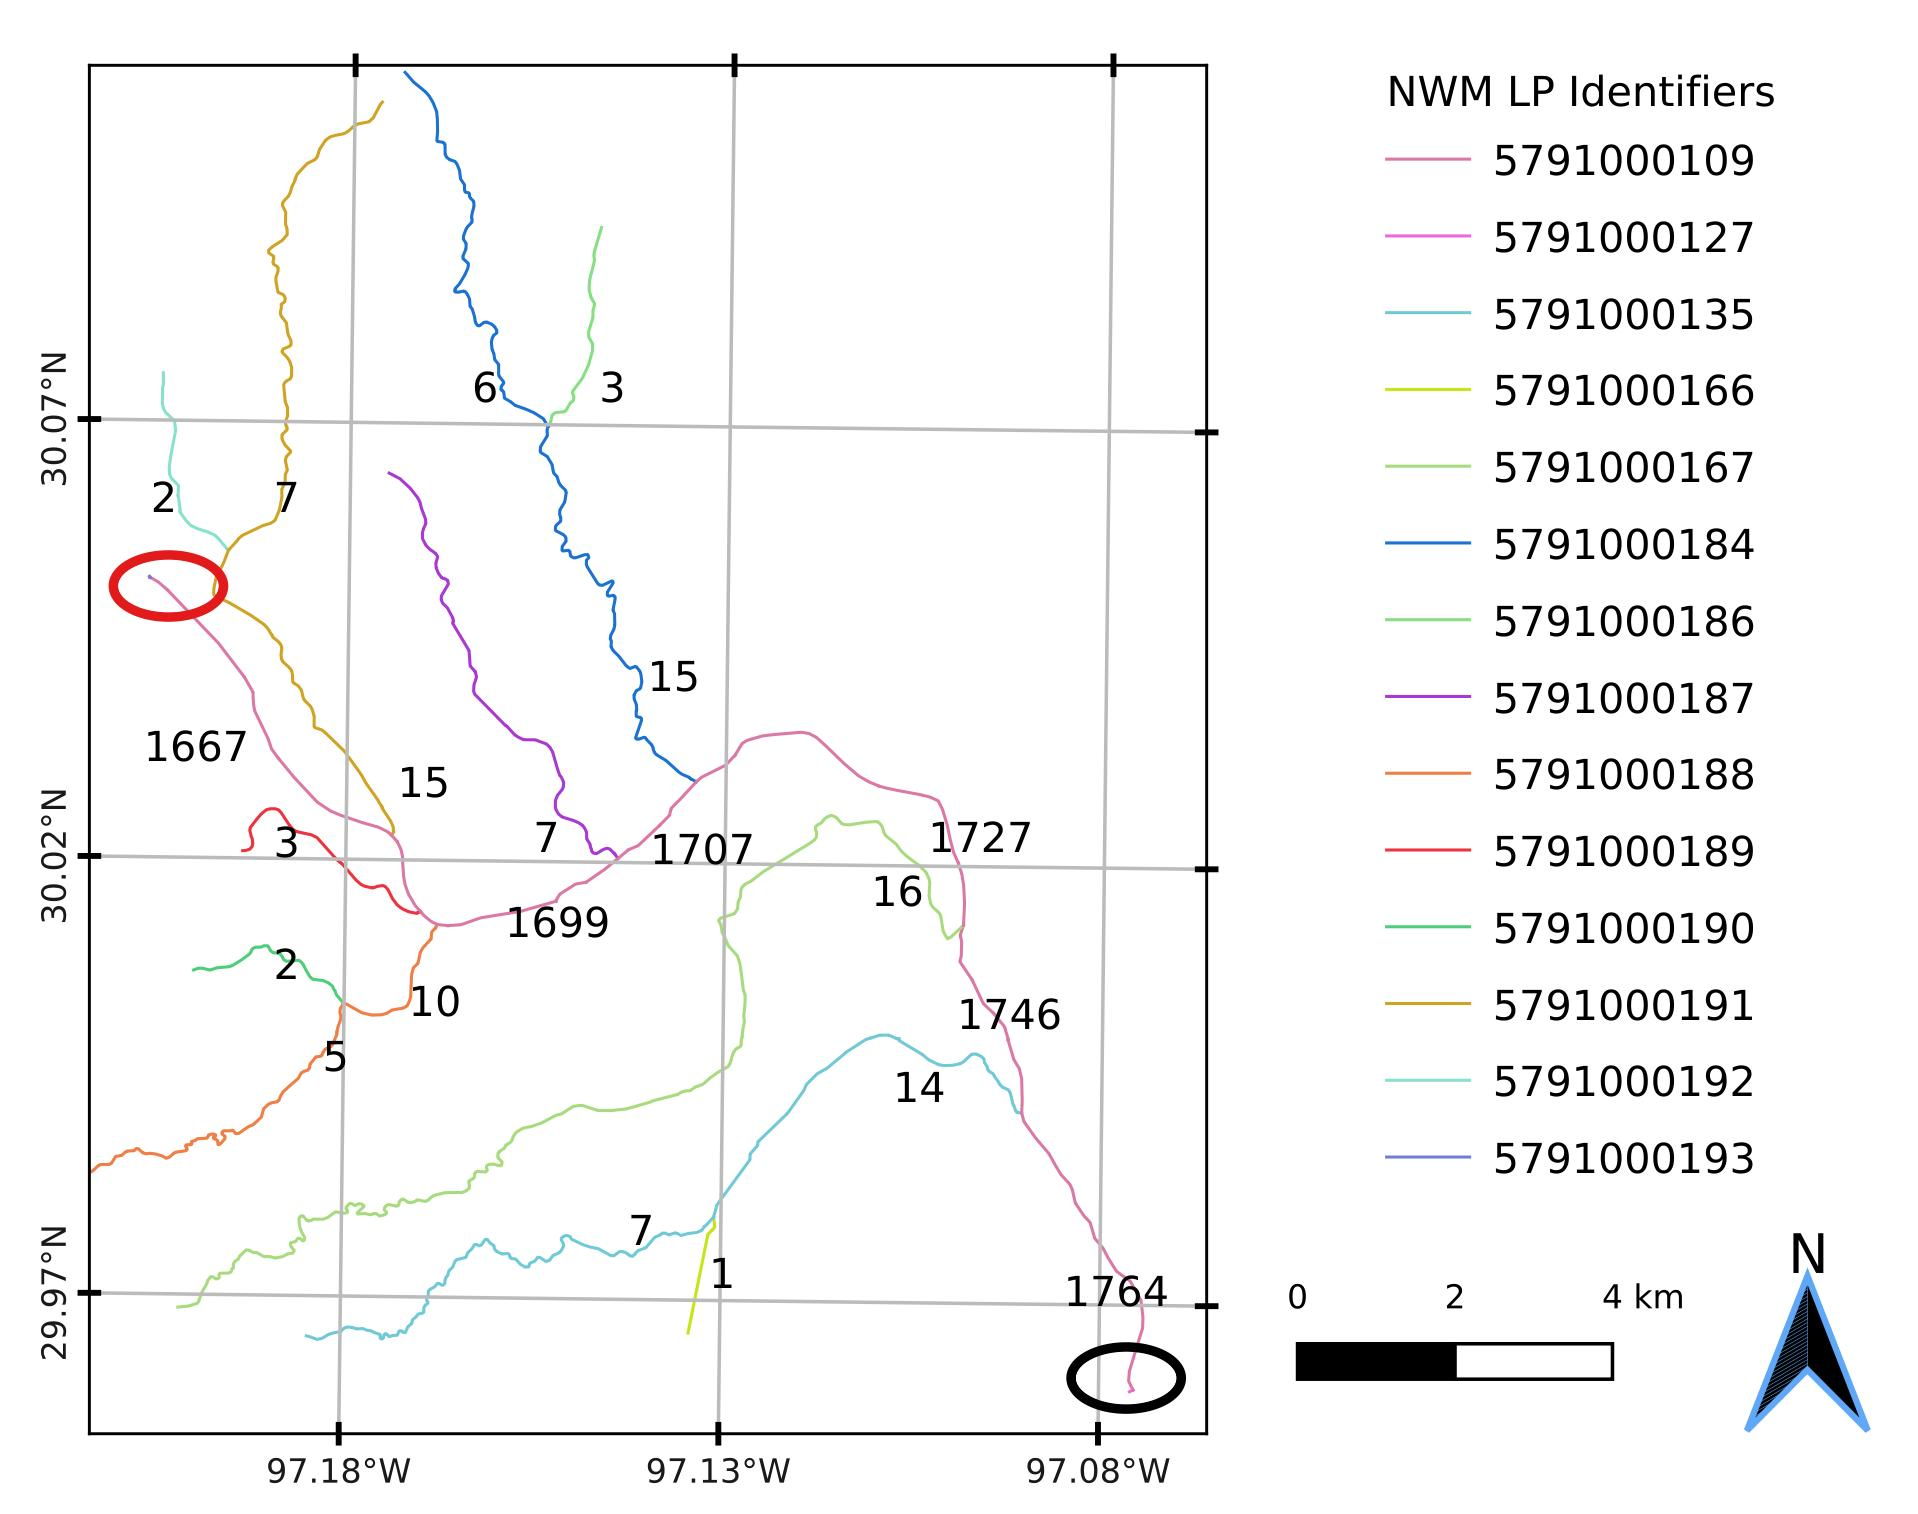
\includegraphics[scale=1.0]{figures/level_path_methods.jpg}
\caption{Illustrates the NWM Full Resolution V2.1 stream network discretized into level paths (LP), symbolized by unique colors, as well as the values of the arbolate sums in km units.
The LPs were derived on a HUC8 level (12020002) but only illustrated for a small, headwater subset of this HUC8 for clarity purposes.
Arbolate sums are defined as the cumulative drainage distances of all upstream stream lines.
Arbolate sums are computed for the NWM network by starting at the headwater points then traversing downstream and adding the distances cumulatively. 
LPs are derived by starting at an outlet point with a unique identifier (ID).
The unique LP ID is propagated upstream until a junction is reached where the current LP ID is propagated in the direction of maximum arbolate sum.
The remaining converging segments at the given junction are each assigned a new unique LP ID and the process is repeated recursively until all reaches have been assigned a LP.
Thus, LP serve as a proxy means of assigning membership to a given river when presented with a confluence.
Each individual LP has a unit Horton-Strahler stream order thus serves as a great method for our proposed technique.
}
\label{fig:level_path_methods}
\end{figure}
%
%
\begin{figure}[H]
\centering
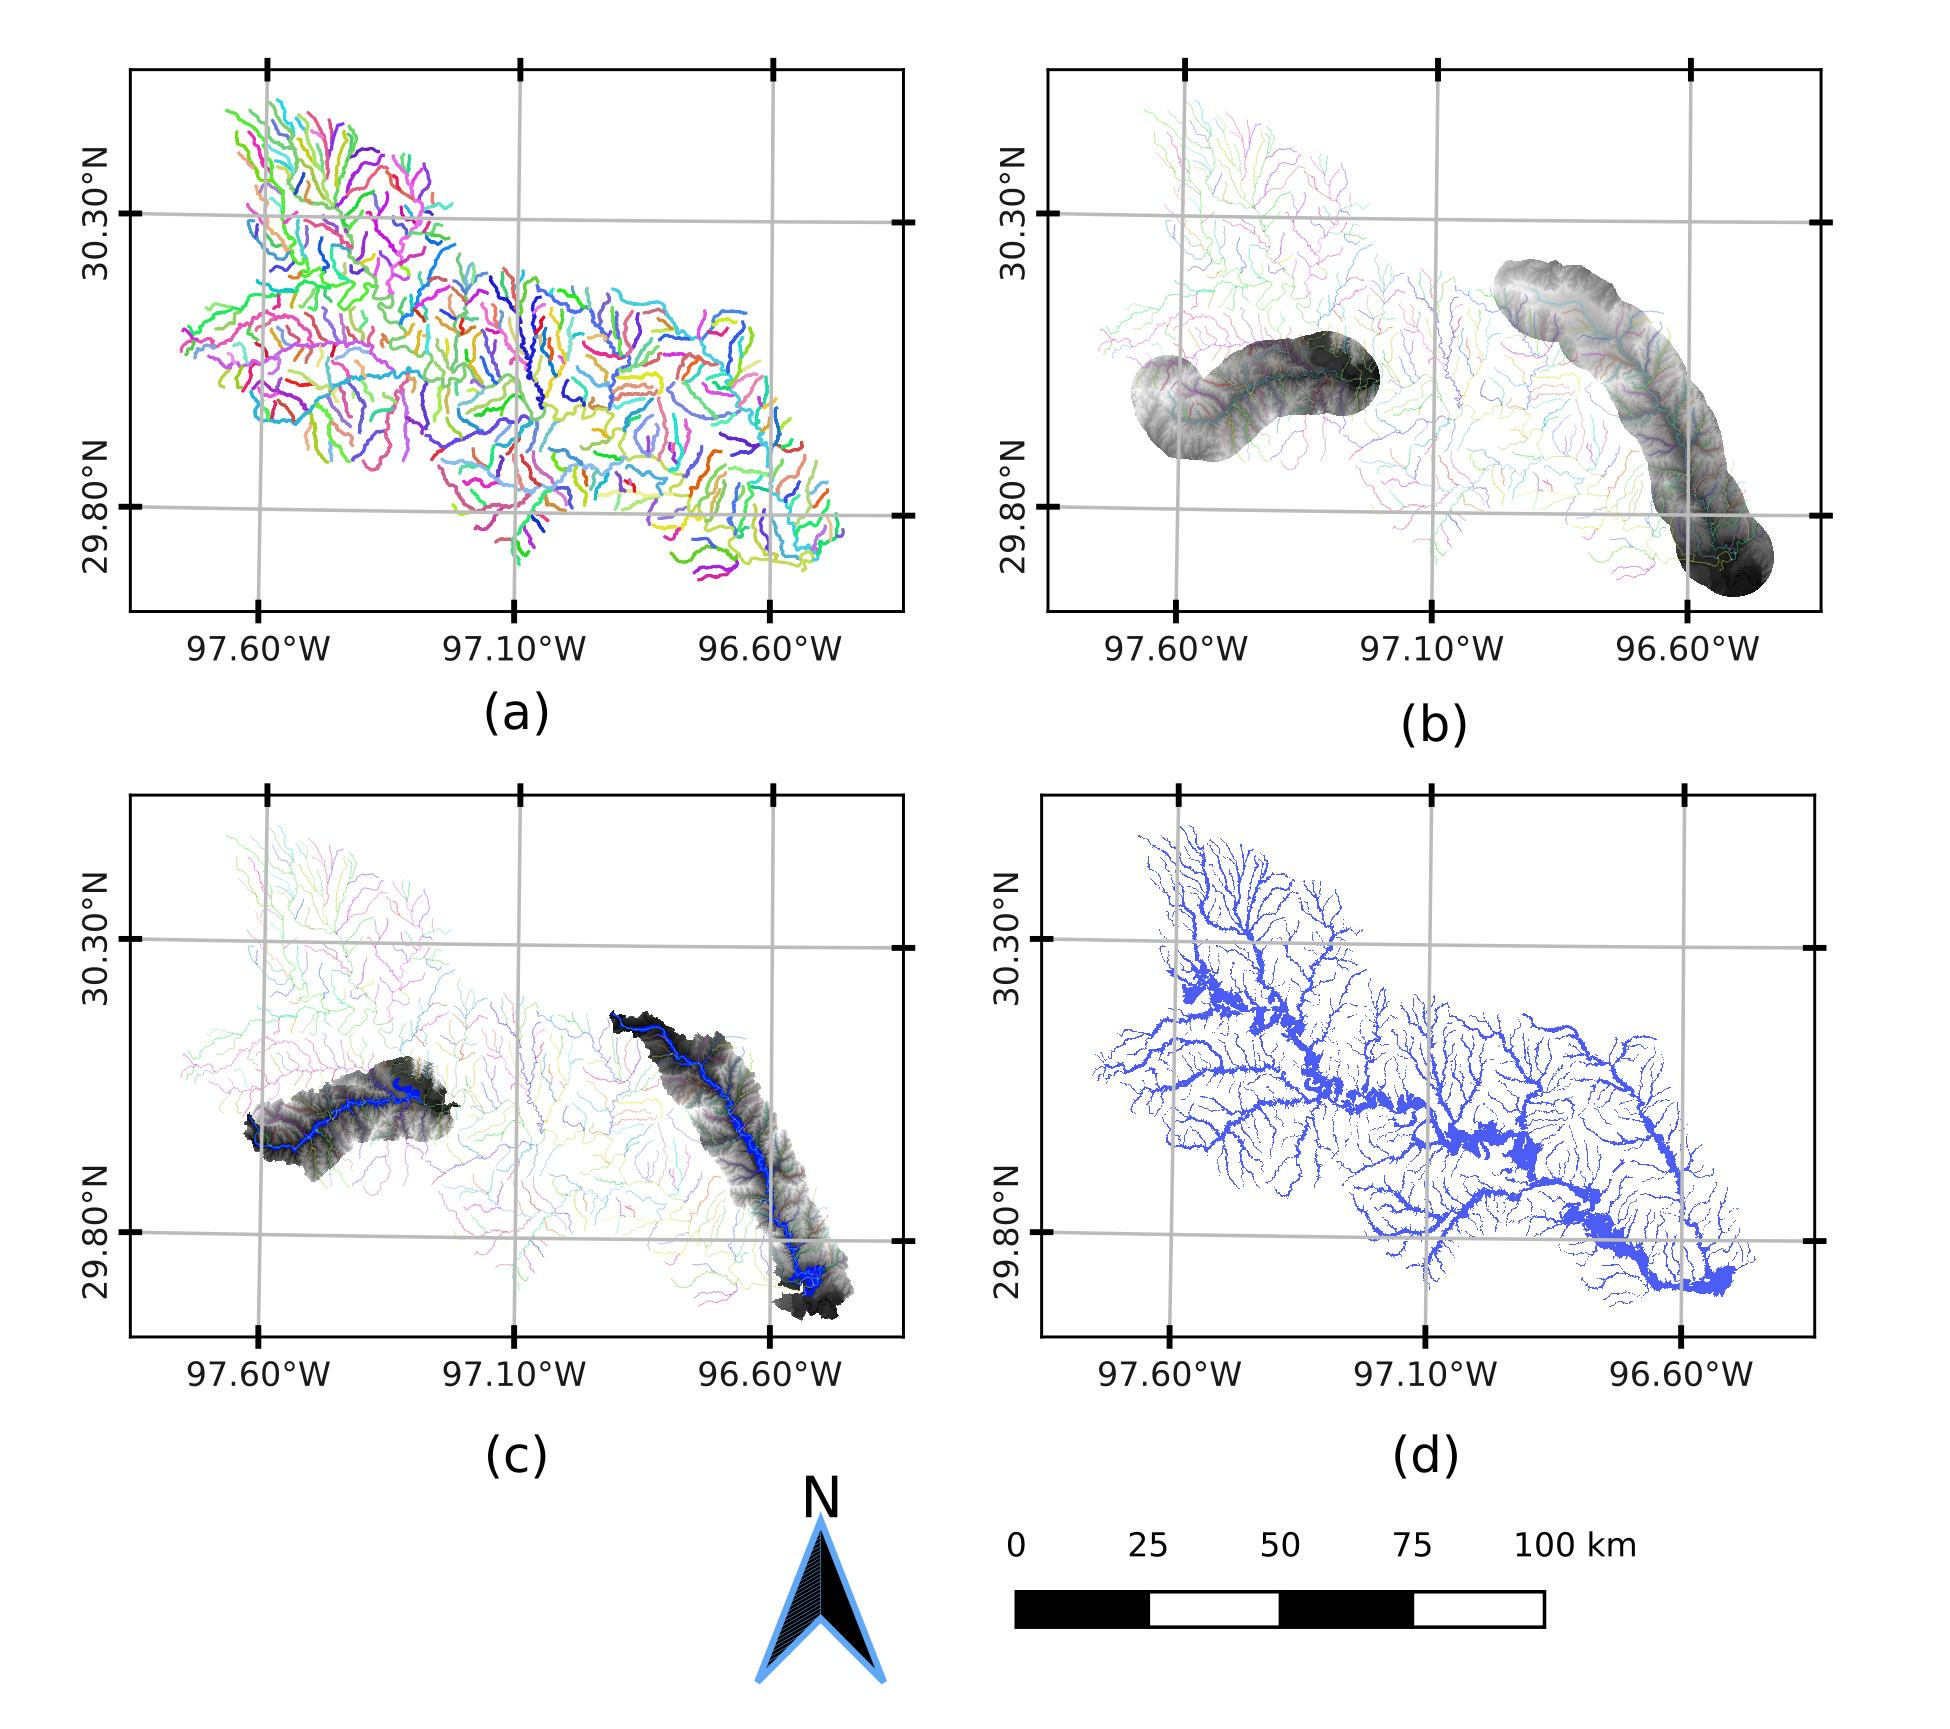
\includegraphics[scale=1.0]{figures/gms_methods.jpg}
\caption{Overall procedure for GMS HAND at HUC8 12090301.
In (a), we illustrate all NWM stream lines symbolized by their LP with 372 unique LP IDs in this HUC.
Meanwhile (b), demonstrates the DEM clipped to a seven km buffer around two selected LPs.
In (c), we show how HAND can be computed just for each one of these two LPs independently. 
We also show inundation maps created for these two LPs in (c). 
In (d), we show all the inundation maps for all the LPs mosaiced together. }
\label{fig:gms_methods}
\end{figure}
%
%
\begin{figure}[H]
\centering
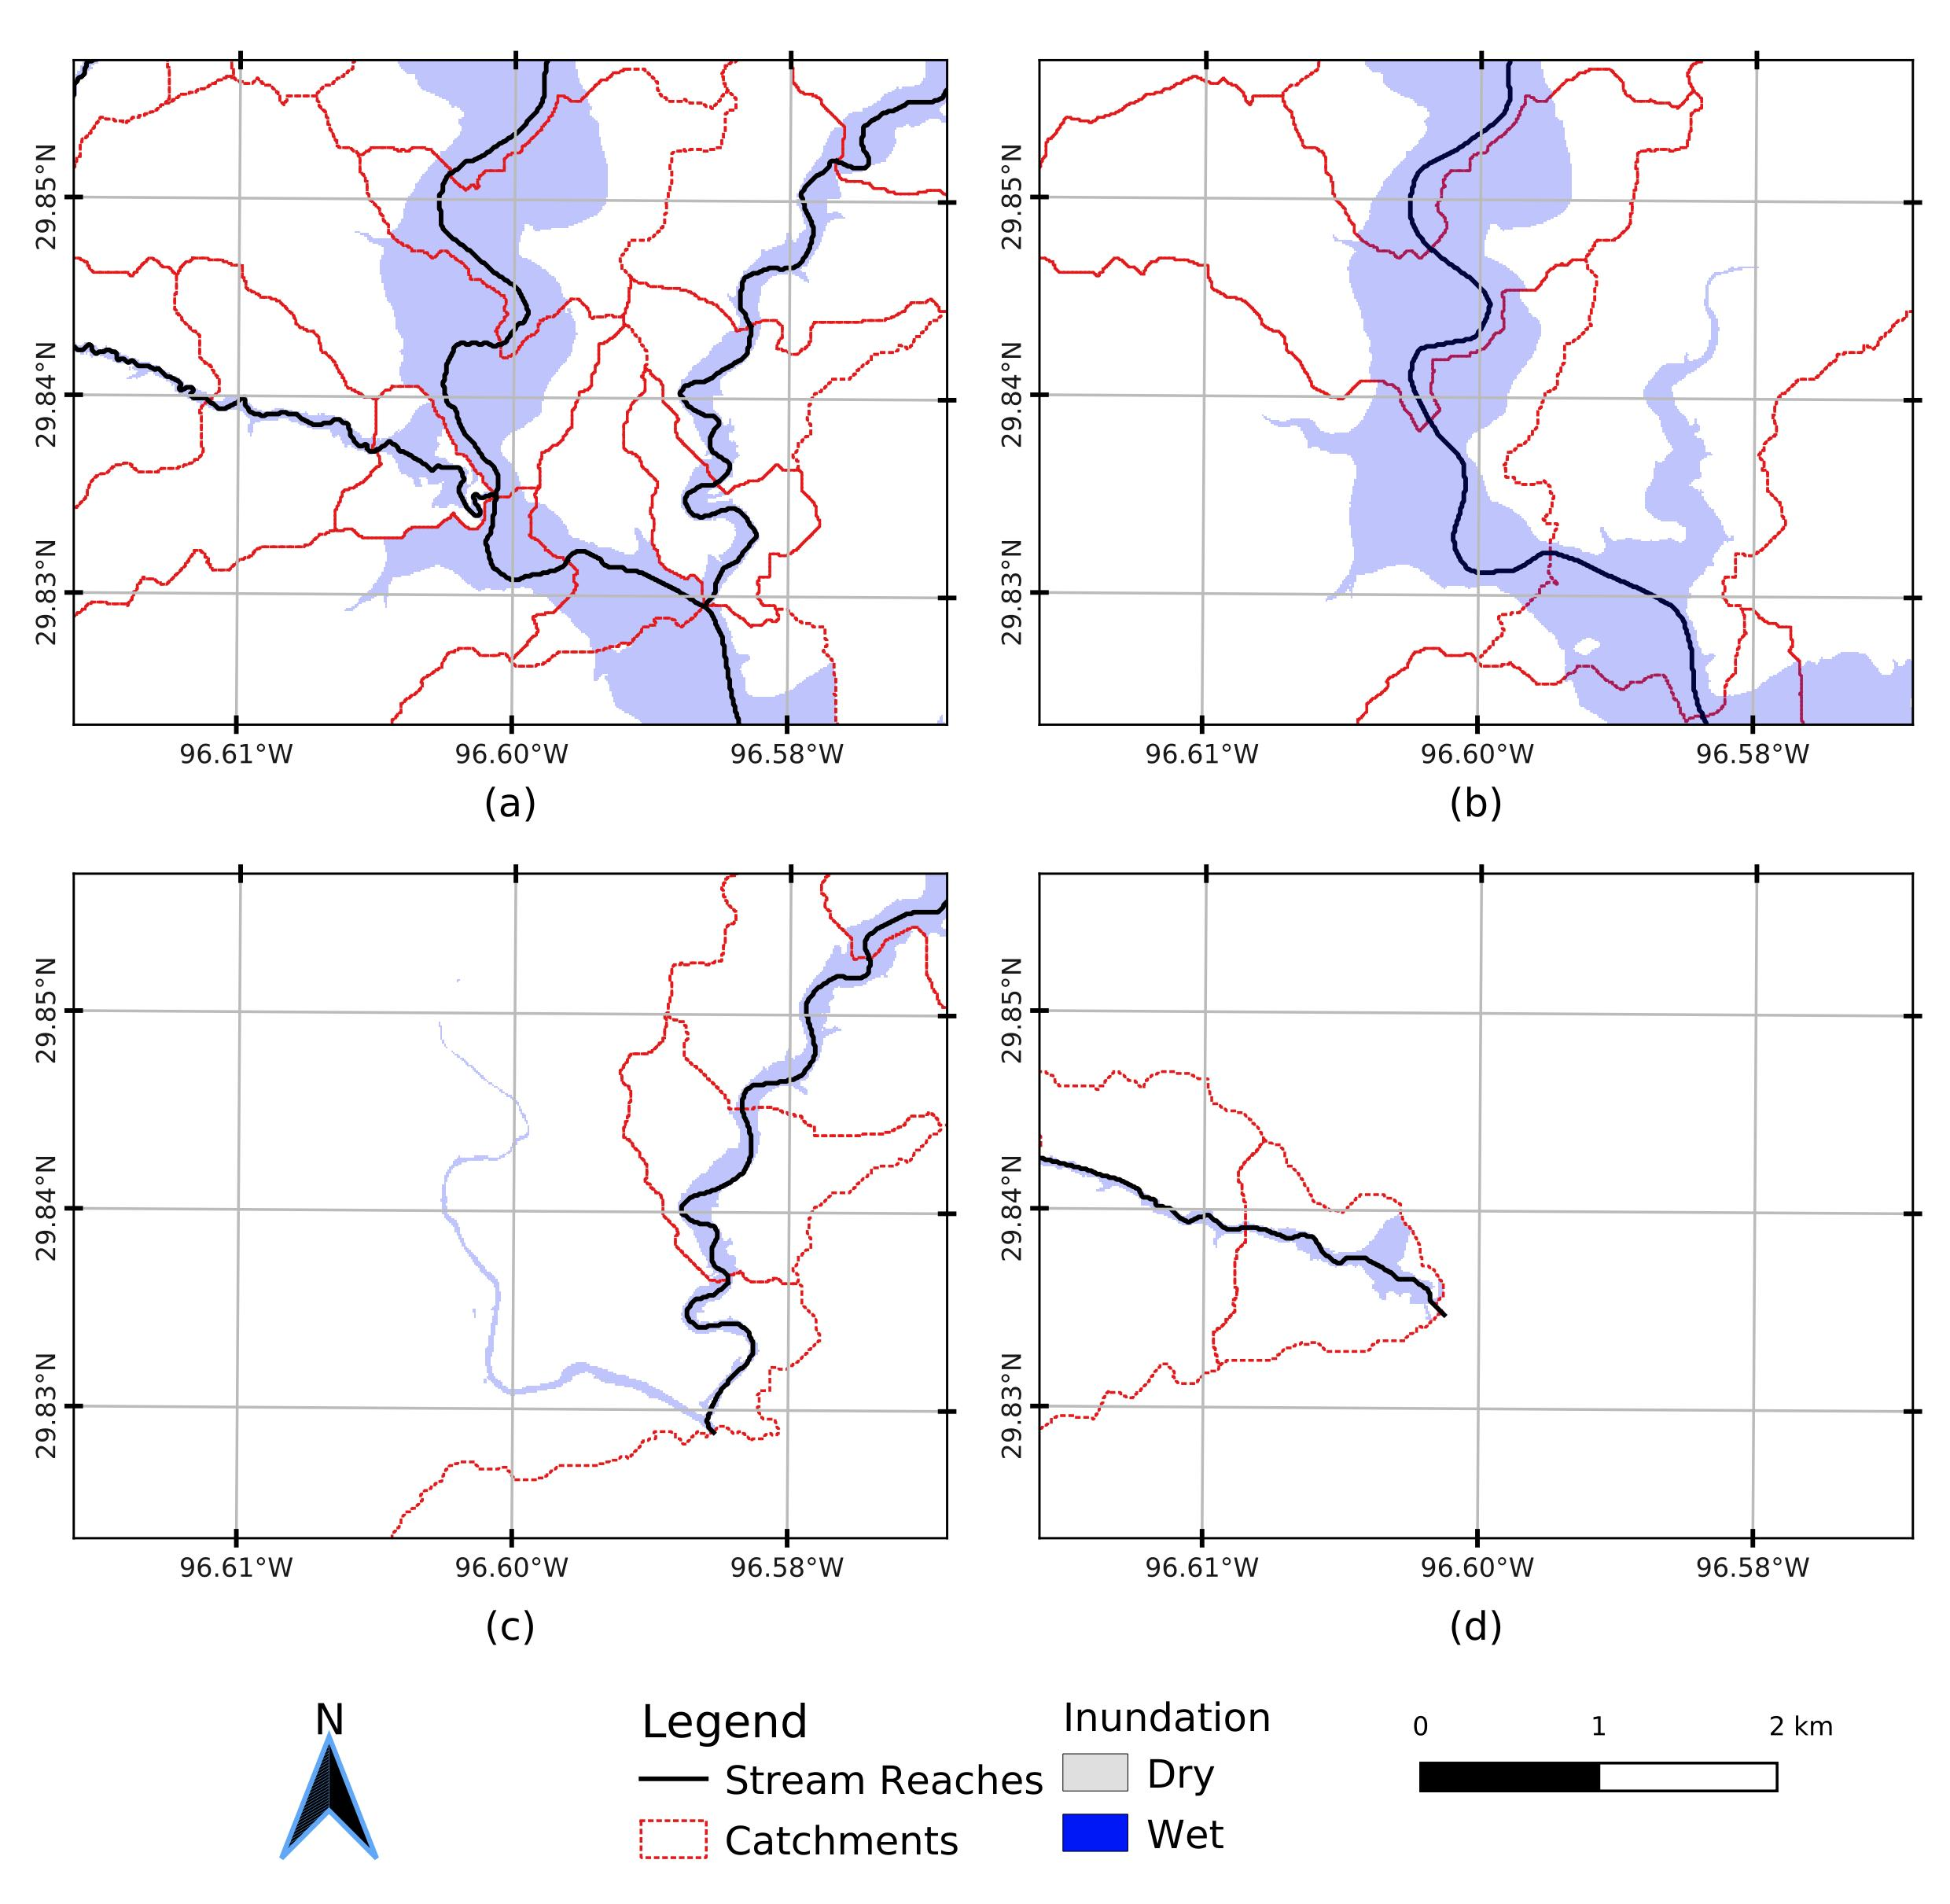
\includegraphics[scale=0.70]{figures/gms_methods_2.jpg}
\caption{This image, with the same spatial domain as Figure \ref{fig:catchment_boundaries_issue} (HUC 12090301), demonstrates how computing HAND on level path (LP) bases leads to larger, independent catchments and more expansive inundation extents (100 yr flows).
In (a), the catchments and stream network are shown for HAND computed in Full-Resolution (FR) method which shows constrained inundation extents around the two junctions.
(b) demonstrates the LP associated with this region's highest order river.
By delineating catchments at this scale independent of the neighboring tributaries, the drainage areas are allowed to expand thus allowing inundation extents to cover previously restricted areas.
In (c) and (d), we show the stream lines, catchments, and inundation extents of the two tributaries.
Later in Section \ref{ssec:inundation_mapping}, we describe how the inundation in (b), (c), and (d) are mosaiced together to form one seamless inundation map.
This process allows for multiple, possible contributing sources of fluvial inundation to be considered thus enhancing FIM skill.
}
\label{fig:gms_methods_2}
\end{figure}
%
%%%%%%%%%%%%%%%%%%%%%%%%%%%%%%%%%%%%%%%%%%%%%%%%%%%%%%%%
\subsection{Inundation Mapping}
\label{ssec:inundation_mapping}
%
The FIM hydrofabric consisting of the relative elevations grid, catchments grid, catchment polygons, rating curve, and cross-walking data are all used to convert forecasts from the NWM into forecasts extents.
For operational situations, one would cache the FIM hydrofabric then either produce libraries of FIM for a sample of discharges or stages or also produce the FIM in near real-time (NRT).
From the cached FIM hydrofabric and design or forecast discharges including those extracted from the NWM, inundation maps can be generated at HUC8 spatial processing units in a rapid, parallel operation. 
The discharges are associated with NWM reach identifiers and cross-walked over to reach identifiers in the FIM hydrofabric.


Utilizing the stage-discharge relationships in the SRCs, each forecast for each catchment identifier is assigned a stage value. 
The catchments grid encoded with the reach identifiers are used to map the stages by thresholding to the forecast stage.
We use the basic logic already established in previous works to conduct this \cite{nobre2016hand,liu2016cybergis,maidment2017conceptual}.
Mathematically, the HAND values, $H_{ij}$, can be indexed by the reach identifiers, i, and pixel indices, j.
For each forecast stage, $S_i$, one can express the formula for $D_{ij}$, a continuous variable denoting water depth at a given pixel with reach and pixel identifiers i and j respectively in Equation \ref{eq:hand_fim_depth}.
While we do not evaluate FIM depths in this study, we do compute depths first as to threshold them to produce extents.
For each forecast stage, $S_i$, one can express the formula for $F_{ij}$, a binary variable denoting inundation condition in Equation \ref{eq:hand_fim} in terms of $D_{ij}$ by simply thresholding at zero depths.
%
\begin{linenomath*}
\begin{equation}
\label{eq:hand_fim_depth}
    D_{ij} = S_i - H_{ij}
\end{equation}
\end{linenomath*}
%
\begin{linenomath*}
\begin{equation}
\label{eq:hand_fim}
    F_{ij} = D_{ij} > 0
\end{equation}
\end{linenomath*}
%
For the cases of MS and GMS, the inundation maps produced for the respective processing units at lower maximum stream orders must be mosaiced together to form a seamless forecast in the form of a single raster file.
For mosaicing the depths, we select the maximum inundation depth from the all the contributing areas K index by its lower case character, k.
Consolidating the depths using a maximum function was decided upon based on intuition which we believe to best represent the depth of water in an area with multiple contributing fluvial inundation sources.
Other aggregation methods could lead to different results but were not investigated here.
Equation \ref{eq:comp_fim_depths} illustrates how the maximum depth from all the contributing areas, k, to each pixel j in catchment i,
%
\begin{linenomath*}
\begin{equation}
\label{eq:comp_fim_depths}
    D_{ij} = \max_{k=[1,...,K]} D_{ijk}
\end{equation}
\end{linenomath*}
%
. Equation \ref{eq:comp_fim} illustrates the same process but for mosaicing the binary inundation maps,
%
\begin{linenomath*}
\begin{equation}
\label{eq:comp_fim}
    F_{ij} = \max_{k=[1,...,K]} F_{ijk}
\end{equation}
\end{linenomath*}
. For the MS and GMS methods, the contributing areas are defined differently.
For MS, the FIM from MS HAND and FR HAND are mosaiced together to form a singular inundation map thus K is set to two for that case.
For GMS, all FIMs from all the LPs in a given area are mosaiced together then K is set to this number of LPs.
Lastly, we apply Equation \ref{eq:hand_fim} to the mosaiced depths for the MS and GMS cases in order to obtain FIM extents which is the subject of our evaluations.
Figures \ref{fig:gms_methods}a and \ref{fig:gms_methods}b, illustrate how inundation maps are created for lower stream order processing units then mosaiced together.
%
%%%%%%%%%%%%%%%%%%%%%%%%%%%%%%%%%%%%%%%%%%%%%%%%%%%%%%%%
\subsection{Evaluation}
\label{ssec:evaluation}
%%%%%%%%%%%%%%%%%%%%%%%%%%%%%%%%%%%%%%%%%%%%%%%%%%%%%%%%
%
OWP FIM is linked with the NWM for operational purposes, utilizing streamflow inputs, to produce FIM at a continental scale.
We evaluated various validation data sources for operational use, each with its own strengths and weaknesses, including high water marks (HWMs) \cite{musser2017characterization,watson2017characterization,breaker2016characterization}, remote sensing observations \cite{aristizabal2020high,aristizabal2021mapping}, and modeled extents from hyper-resolution, local models \cite{mcenery2005noaa}.
Although they have advantages, the three data sources mentioned do not have streamflow information, which is required by OWP FIM.
Using the NWM as a source of streamflow input would be a logical choice due to its operational use, but this would introduce hydro-climatic uncertainties that could impact the results of adding a multi-fluvial source extension to HAND.
On the other hand, relying on point sources of streamflow or stage, such as gages, would eliminate this limitation, but limit the information available to only a single source of inundation at a specific site.
Given these limitations, we investigated the use of existing HEC-RAS based models to address the limitations caused by hydro-climatic uncertainties and sparse streamflow inputs.

Our HAND based approach coupled with SRCs requires streamflow as input and is agnostic as to the source of that streamflow whether forecasted, observed, or probablistic.
Due to this fact, evaluation of our relative elevation CFIM method was conducted by comparison to the HEC-RAS 1D models produced within FEMA region 6 \cite{fema2021base,fema2021estimated,us2022hydrologic}.
This dataset was selected due to its large spatial coverage, availability of cross-sections with streamflow information, higher level of sophistication when compared to HAND, engineering scale detail, and a storied use in the literature as an evaluation dataset \cite{cook2009effect,rajib2016large,zheng2018geoflood,afshari2018comparison,wing2017validation,criss2022stage,follum2017autorapid,bates201630m,wing2017validation,hu2021real,li2022accounting,li2022comprehensive,zheng2018geoflood}.
We selected 49 available HUC8s, shown in Figure \ref{fig:all_ble_maps}, which span about 185 thousand $km^2$ across nine states.
The maps of the 1\% recurrence flow (1 in 100 year) and the 0.2\% recurrence flow (1 in 500 year) are furnished by InFRM as well as the corresponding discharges and mapping extents for evaluation.
We did exclude NWM V2.1 Reservoirs from evaluation because these are not properly accounted for in the inundation sourced from OWP FIM.
Since the BLE does account for reservoir inundation, some of the BLE reservoir inundation extents extend beyond the NWM reservoir geometries contributing to false negatives (FNs), or under-prediction.

By using the same HEC-RAS derived discharges and FIM extents for creating maps with OWP FIM, we are able to separate out errors introduced by NWM inputs and processes including land surface interactions, groundwater fluxes, atmospheric forcings, hydraulic routing, and others that would have potentially affected our conclusions if we had used NWM forecasted discharges.
Figure \ref{fig:ble_evaluation_method} illustrates both NWM V2.1 and BLE stream lines as well as the BLE cross-sections that have recurrence discharges associated with them.
We elected to spatially intersect the HEC-RAS cross sections with the NWM stream network assigning the 1\% and 0.2\% flow rates to each NWM reach. 
To handle multiple intersections, we opted to use a filter to select the median discharge value attributed to each NWM reach.
This partially handles the influence of neighboring cross sections that could cause flow discontinuities and mass conservation issues.
Additionally, the stream network of the InFRM furnished models are of higher stream densities and bifurcation ratios, as evident in Figure \ref{fig:ble_evaluation_method}, leading to a significant amount of FNs along headwater streams with unit Horton-Strahler order due to the lack of representation of these additional headwater streams in the NWM network.
While the limitations are noted, this method does best to detangle the influence of exogenous variables that we do not wish to study in this comparison.
%
\begin{figure}[H]
\centering
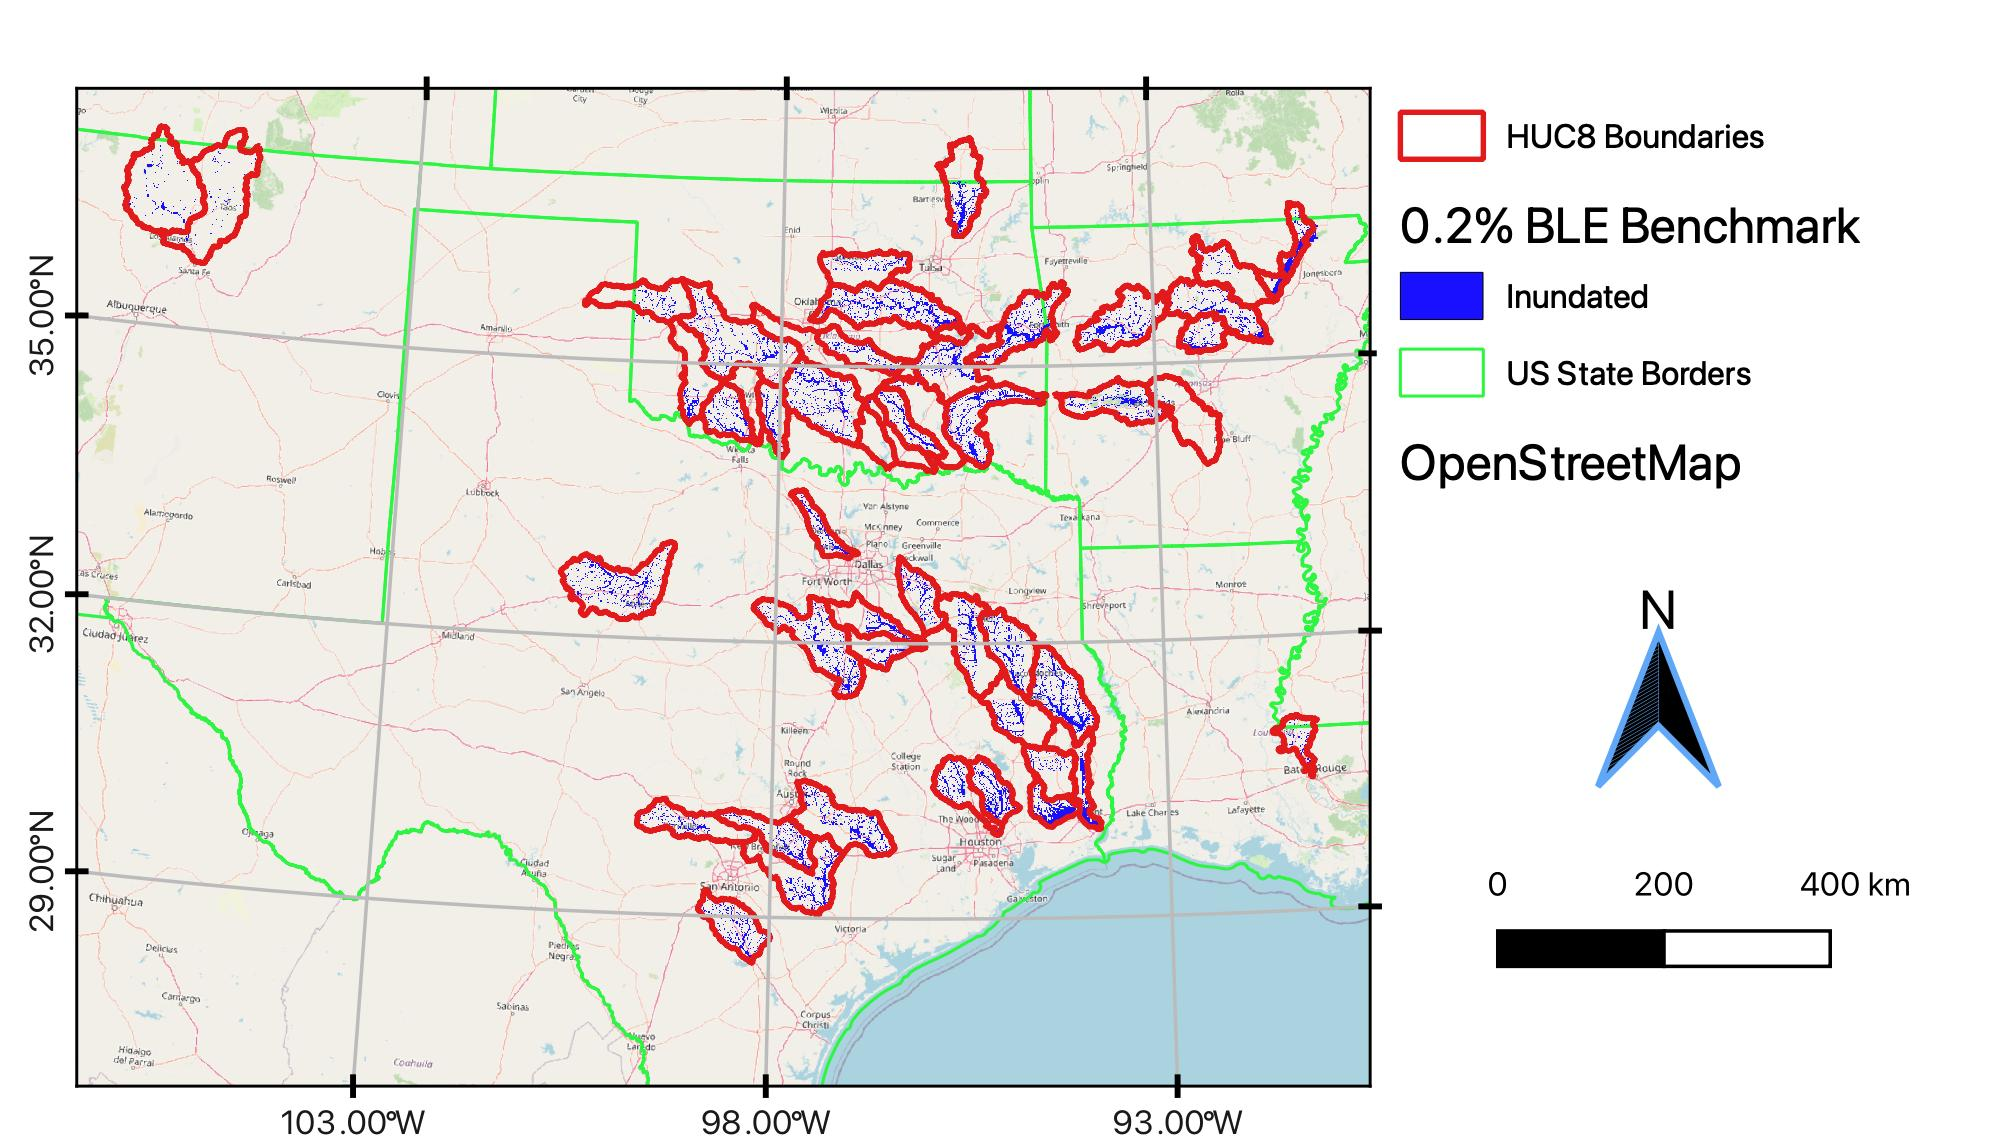
\includegraphics[scale=1.0]{figures/all_ble_maps.jpg}
\caption{
Shows 185 thousand $km^2$ of modeled areas for the Base Level Engineering (BLE) domain of 49 HUC8s across nine states at 0.2\% recurrence magnitude for flow rates.
BLE maps are produced for two recurrence flows, 1\% (100 yr) and 0.2\% (500 yr), using 1D HEC-RAS models.
The maps are used as benchmarks for validation purposes of OWP FIM.
}
\label{fig:all_ble_maps}
\end{figure}
%
\begin{figure}[H]
\centering
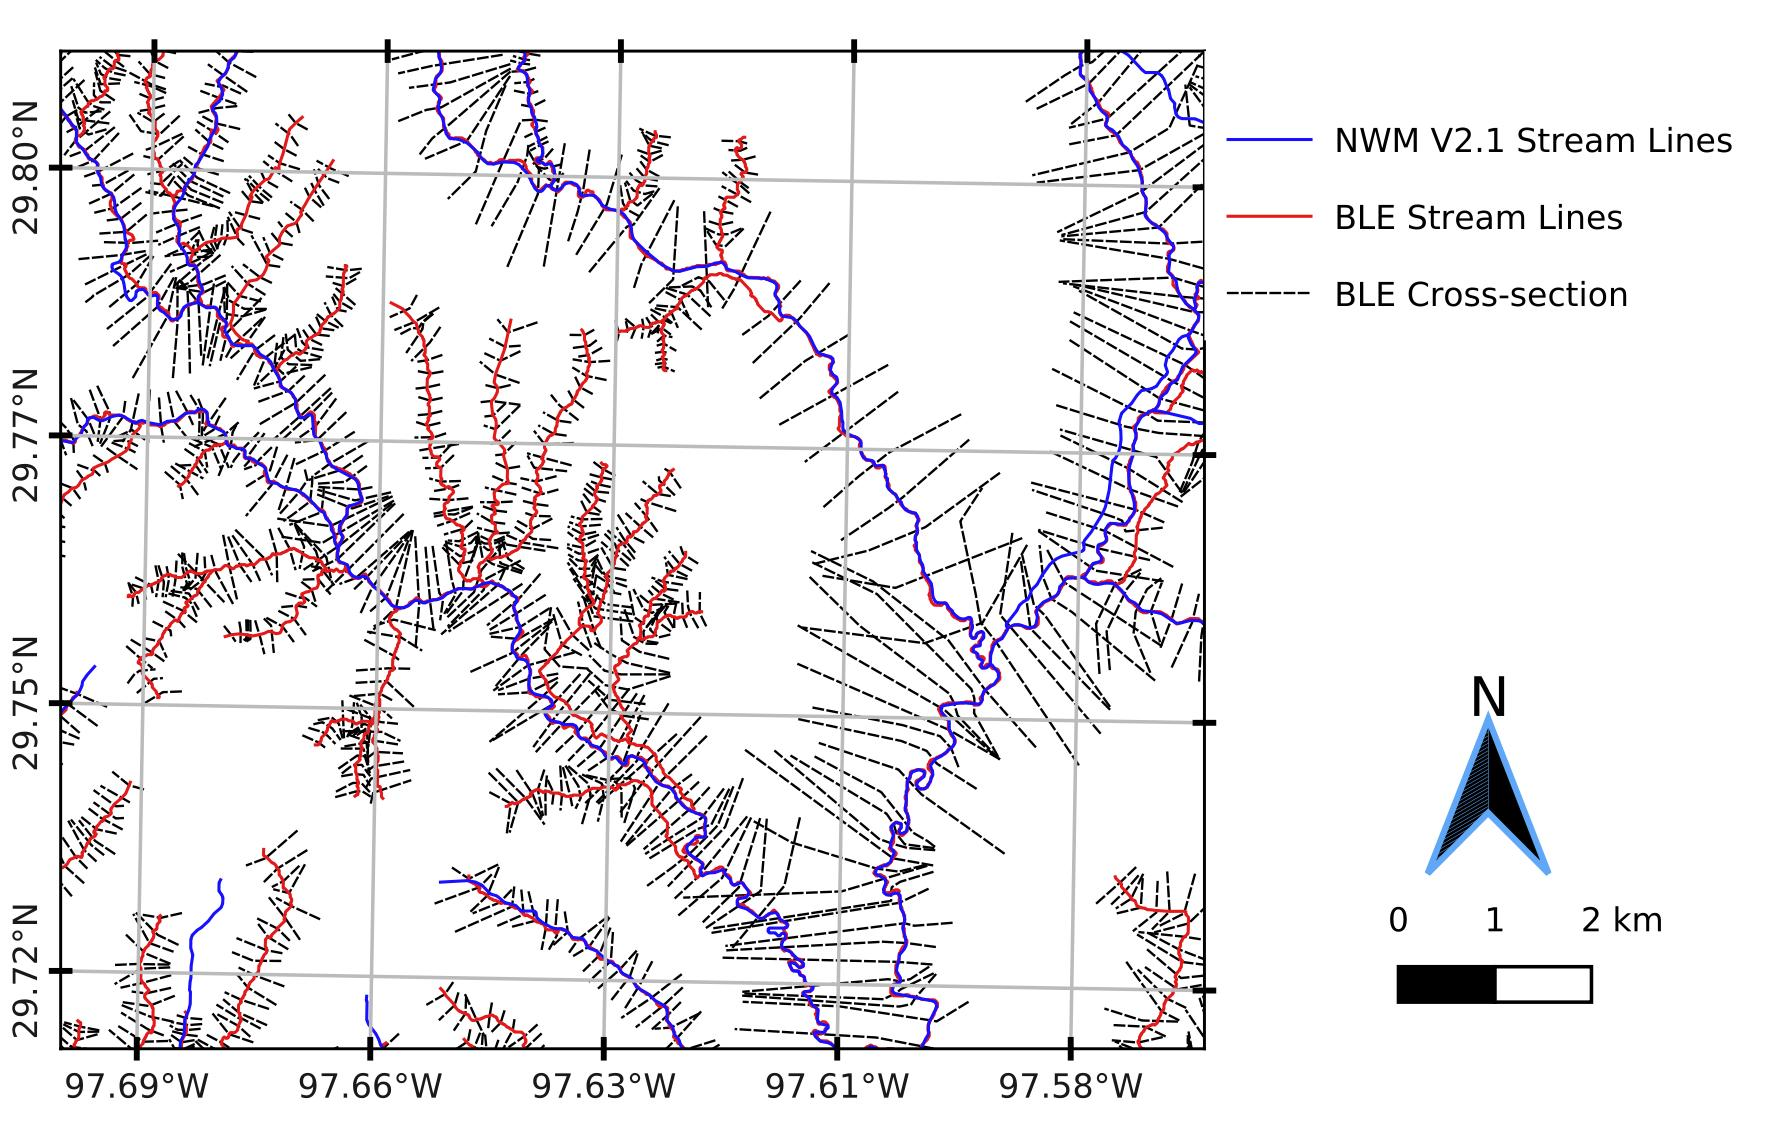
\includegraphics[scale=1.0]{figures/ble_evaluation_method.jpg}
\caption{
Illustrates Base Level Engineering (BLE) cross sections and stream lines at the HUC8 12100203 near the confluences of West Fork Plum Creek and Clear Fork Plum Creek with Plum Creek.
BLE cross sections are intersected with NWM reaches and the median recurrence discharge for 1\% and 0.2\% levels are selected per NWM V2.1 Full Resolution (FR) stream lines.
Additionally, we illustrate the NWM V2.1 catchments to provide a sense of how many cross-sections may intersect a given NWM flowline.
The BLE stream network is also shown which is denser than the NWM V2.1 stream lines meaning there are several lower order streams represented in the BLE stream network that are not in the NWM V2.1 stream lines.
This creates additional inundation areas in the validation data that are not modeled with our HAND based FIMs.
}
\label{fig:ble_evaluation_method}
\end{figure}
%

The metrics employed in this study to evaluate inundation extents include CSI, Probability of Detection (POD), and False Alarm Ratio (FAR) and are presented in Equations \ref{eq:csi}, \ref{eq:pod}, \ref{eq:far}, respectively.
To calculate these secondary metrics, one must define three primary metrics starting with true positives (TP) which is predicted wet and wet in the BLE benchmark dataset.
The two types of errors consist of false positives (FP), or type I errors, which is dry in the benchmark but predicted wet and false negatives (FN), or type II errors, which is wet in the benchmark but predicted dry. 
Lastly, the reader may come across true negatives (TN) which is defined as dry in both the benchmark and predicted datasets.
Maximizing POD indicates a model's ability to detect the given threat of interest, inundation, while minimizing FAR is sought to indicate a models ability in reducing FN errors.
In other words, POD is an indicator of model skill in inundated regions while FAR is an indicator of model skill in non-inundated regions.
Some work by \citeA{gerapetritis2004behavior} denotes CSI a good proxy for measuring a forecasting system's utility in protecting life and property and has been shown to be optimized mathematically when $POD = 1 - FAR$.
We use all three secondary metrics here to add value to the discussion while avoiding aggregating away the meaning of all four primary metrics.

While these metrics are commonly employed in the evaluation of FIM and binary weather prediction communities in general, they do come with some notable limitations including frequency dependence in the case of CSI and FAR \cite{gerapetritis2004behavior,stephens2014problems,schaefer1990critical,jolliffe2012forecast}.
Thus, frequency dependent statistics should be used with caution when comparing across sites with varying frequencies. 
Lastly, approximately six HUC8s do not have NWM MS reaches thus we imputed the metrics for FR for these sites as the best available forecasting capability to compare GMS metrics to.
%
\begin{linenomath*}
\begin{equation}
\label{eq:csi}
CSI = \frac{TP}{TP + FN + FP}
\end{equation}
\end{linenomath*}
%
\begin{linenomath*}
\begin{equation}
\label{eq:pod}
POD = \frac{TP}{TP + FN}
\end{equation}
\end{linenomath*}
%
\begin{linenomath*}
\begin{equation}
\label{eq:far}
FAR = \frac{FP}{TP + FP}
\end{equation}
\end{linenomath*}
%
